\documentclass[aspectratio=169,10pt]{beamer}

\usepackage[T1]{fontenc}
\usepackage{lmodern}
\usepackage{tikz}
\usepackage{listings}
\usepackage{booktabs}
\usepackage{array}
\usepackage{microtype}

\definecolor{navy}{HTML}{08091F}
\definecolor{panel}{HTML}{151832}
\definecolor{panelalt}{HTML}{1C2040}
\definecolor{white}{HTML}{F7F8FC}
\definecolor{muted}{HTML}{BEC4D9}
\definecolor{cyan}{HTML}{55D6E8}
\definecolor{coral}{HTML}{FF647C}
\definecolor{mint}{HTML}{9DE3C3}
\definecolor{lavender}{HTML}{B5A5FF}
\definecolor{grid}{HTML}{3A4164}

\setbeamertemplate{navigation symbols}{}
\setbeamertemplate{itemize item}{\color{cyan}\raisebox{0.15ex}{\small$\blacktriangleright$}}
\setbeamertemplate{itemize subitem}{\color{coral}\tiny$\bullet$}
\setbeamercolor{normal text}{fg=white,bg=navy}
\setbeamercolor{background canvas}{bg=navy}
\setbeamercolor{frametitle}{fg=white,bg=navy}
\setbeamercolor{block title}{fg=white,bg=panelalt}
\setbeamercolor{block body}{fg=white,bg=panel}
\setbeamerfont{frametitle}{size=\Large,series=\bfseries}
\setbeamersize{text margin left=0.55cm,text margin right=0.55cm}

\setbeamertemplate{background canvas}{
  \begin{tikzpicture}[remember picture,overlay]
    \fill[navy] (current page.south west) rectangle (current page.north east);
    \fill[cyan,opacity=.055] ([xshift=-1.5cm,yshift=-.4cm]current page.north east) circle (4.4cm);
    \fill[coral,opacity=.035] ([xshift=.4cm,yshift=1.1cm]current page.south east) circle (3.4cm);
    \draw[grid,opacity=.35,line width=.35pt]
      ([xshift=.48cm,yshift=-.93cm]current page.north west) --
      ([xshift=-.48cm,yshift=-.93cm]current page.north east);
  \end{tikzpicture}
}

\setbeamertemplate{frametitle}{
  \vspace{.16cm}
  \insertframetitle
  \vspace{.10cm}
}
\setbeamertemplate{footline}{
  \leavevmode
  \hbox{
    \begin{beamercolorbox}[wd=.74\paperwidth,ht=2.7ex,dp=1.1ex,leftskip=.28cm]{normal text}
      \color{muted}\scriptsize HPC \textbullet\ OpenMP \textbullet\ LU decomposition
    \end{beamercolorbox}
    \begin{beamercolorbox}[wd=.26\paperwidth,ht=2.7ex,dp=1.1ex,rightskip=.15cm]{normal text}
      \color{cyan}\scriptsize TEAM 6 \hfill
      \color{muted}\number\numexpr\insertframenumber+6\relax/21
    \end{beamercolorbox}
  }
}

\lstset{
  language=C,
  basicstyle=\ttfamily\scriptsize\color{white},
  keywordstyle=\color{cyan}\bfseries,
  commentstyle=\color{muted}\itshape,
  stringstyle=\color{mint},
  showstringspaces=false,
  breaklines=true,
  columns=fullflexible,
  keepspaces=true,
  aboveskip=.15em,
  belowskip=.15em,
  xleftmargin=.15em,
  frame=none
}

\newcommand{\eyebrow}[1]{%
  {\color{cyan}\scriptsize\bfseries #1}\par\vspace{.08cm}}
\newcommand{\smallmuted}[1]{{\color{muted}\small #1}}
\newcommand{\metric}[2]{%
  {\color{#1}\Large\bfseries #2}}
\newcommand{\cardtitle}[2]{%
  {\color{#1}\bfseries\small #2}\par\vspace{.08cm}}
\begin{document}

\begin{frame}[fragile]{After SIMD: remove redundant work}
  \eyebrow{CUMULATIVE OPTIMIZATIONS \quad / \quad 01}
  {\smallmuted{SIMD exposes parallel instructions; the next steps reduce what each iteration has to do.}}
  \vspace{.12cm}

  \begin{columns}[T,onlytextwidth]
    \begin{column}{.485\textwidth}
      \begin{beamercolorbox}[rounded=true,sep=.22cm,wd=\textwidth]{block body}
        \cardtitle{coral}{01 \quad RECIPROCAL OF THE PIVOT}
        {\smallmuted{The pivot is constant while the whole row is normalized.}}
        \vspace{.08cm}
\begin{lstlisting}
inv = 1.0 / A[k][k];   // once per thread, per k
#pragma omp for simd
for (j = k + 1; j < n; ++j)
    A[k][j] *= inv;
\end{lstlisting}
        \vspace{.05cm}
        \small Replaces repeated element-wise divisions with a reusable
        reciprocal and multiplications. Fewer expensive operations can help
        the compiler vectorize the loop.
      \end{beamercolorbox}
    \end{column}
    \begin{column}{.485\textwidth}
      \begin{beamercolorbox}[rounded=true,sep=.22cm,wd=\textwidth]{block body}
        \cardtitle{mint}{02 \quad HOIST A LOOP-INVARIANT LOAD}
        {\smallmuted{\texttt{A[i][k]} does not change as column \texttt{j} advances.}}
        \vspace{.08cm}
\begin{lstlisting}
aik = A[i][k];         // once per row
for (j = k + 1; j < n; ++j)
    A[i][j] -= aik * A[k][j];
\end{lstlisting}
        \vspace{.05cm}
        \small Reuses one value across the row update instead of expressing
        a load in every iteration. An optimizing compiler may already hoist
        it, so the generated code must be checked.
      \end{beamercolorbox}
    \end{column}
  \end{columns}

  \vspace{.2cm}
  \begin{beamercolorbox}[rounded=true,sep=.12cm,wd=\textwidth]{block body}
    \centering\small
    \color{cyan}\textbf{Goal:} reduce scalar work \quad
    \color{muted}$\rightarrow$\quad
    \color{mint}\textbf{leave a simpler, vector-friendly inner loop}
  \end{beamercolorbox}
\end{frame}

\begin{frame}[fragile]{Expose contiguous rows and non-aliasing}
  \eyebrow{CUMULATIVE OPTIMIZATIONS \quad / \quad 02}
  {\smallmuted{The update is a streaming operation across columns of two distinct rows.}}
  \vspace{.1cm}

  \begin{columns}[T,onlytextwidth]
    \begin{column}{.53\textwidth}
      \begin{beamercolorbox}[rounded=true,sep=.22cm,wd=\textwidth]{block body}
        \cardtitle{cyan}{ROW UPDATE}
        \begin{center}
          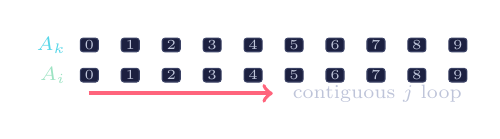
\begin{tikzpicture}[x=.52cm,y=.48cm]
            \foreach \x in {0,...,9} {
              \draw[fill=panelalt,draw=grid,rounded corners=1pt] (\x,1.35) rectangle ++(.44,.36);
              \draw[fill=panelalt,draw=grid,rounded corners=1pt] (\x,.55) rectangle ++(.44,.36);
              \node[font=\tiny,text=muted] at (\x+.22,1.53) {\x};
              \node[font=\tiny,text=muted] at (\x+.22,.73) {\x};
            }
            \node[anchor=east,font=\scriptsize\bfseries,text=cyan] at (-.12,1.53) {$A_k$};
            \node[anchor=east,font=\scriptsize\bfseries,text=mint] at (-.12,.73) {$A_i$};
            \draw[->,line width=1.4pt,coral] (.2,.25) -- (4.7,.25);
            \node[anchor=west,font=\scriptsize,text=muted] at (4.95,.25) {contiguous $j$ loop};
          \end{tikzpicture}
        \end{center}
\begin{lstlisting}
double aik = A[i][k];
double *restrict Ai = A[i];
const double *restrict Ak = A[k];
#pragma omp simd
for (j = k + 1; j < n; ++j)
    Ai[j] -= aik * Ak[j];
\end{lstlisting}
      \end{beamercolorbox}
    \end{column}
    \begin{column}{.445\textwidth}
      \begin{beamercolorbox}[rounded=true,sep=.22cm,wd=\textwidth]{block body}
        \cardtitle{lavender}{WHY THESE POINTERS HELP}
        \begin{itemize}
          \item Row pointers make the linear access pattern explicit.
          \item \texttt{restrict} tells the compiler that \texttt{Ai} and
                \texttt{Ak} do not overlap.
          \item Here, $i>k$: the updated row and pivot row are distinct.
          \item This can help vector loads/stores and code reordering.
        \end{itemize}
        \vspace{.02cm}
        \begin{beamercolorbox}[rounded=true,sep=.08cm,wd=\textwidth]{block title}
          \color{coral}\scriptsize CONTRACT \quad
          \color{white}\scriptsize A false \texttt{restrict} promise causes
          undefined behavior.
        \end{beamercolorbox}
      \end{beamercolorbox}
    \end{column}
  \end{columns}
  \vspace{.06cm}
  \centering\smallmuted{SIMD directives permit vector execution; the compiler decides whether to emit vector instructions.}
\end{frame}

\begin{frame}{Scheduling: contiguous blocks vs. cyclic rows}
  \eyebrow{WORK DISTRIBUTION \quad / \quad 03}
  {\smallmuted{The update distributes independent rows for each pivot $k$.}}
  \vspace{.1cm}

  \begin{columns}[T,onlytextwidth]
    \begin{column}{.485\textwidth}
      \begin{beamercolorbox}[rounded=true,sep=.2cm,wd=\textwidth]{block body}
        \cardtitle{cyan}{\texttt{schedule(static)} \quad BLOCKS}
        \smallmuted{Typical assignment: each thread receives a contiguous chunk.}
        \vspace{.06cm}
        \begin{center}
          \begin{tabular}{c|c}
            \textcolor{cyan}{Thread} & Rows handled \\\midrule
            T0 & \textcolor{cyan}{R0 \quad R1}\\
            T1 & \textcolor{coral}{R2 \quad R3}\\
            T2 & \textcolor{mint}{R4 \quad R5}\\
            T3 & \textcolor{lavender}{R6 \quad R7}
          \end{tabular}
        \end{center}
        \small Contiguous ownership can help locality and keeps scheduling
        overhead low.
      \end{beamercolorbox}
    \end{column}
    \begin{column}{.485\textwidth}
      \begin{beamercolorbox}[rounded=true,sep=.2cm,wd=\textwidth]{block body}
        \cardtitle{coral}{\texttt{schedule(static,1)} \quad CYCLIC}
        \smallmuted{Chunk size 1: assign one row at a time in round-robin order.}
        \vspace{.06cm}
        \begin{center}
          \begin{tabular}{c|c}
            \textcolor{cyan}{Thread} & Rows handled \\\midrule
            T0 & \textcolor{cyan}{R0 \quad R4}\\
            T1 & \textcolor{coral}{R1 \quad R5}\\
            T2 & \textcolor{mint}{R2 \quad R6}\\
            T3 & \textcolor{lavender}{R3 \quad R7}
          \end{tabular}
        \end{center}
        \small Can spread uneven work; may scatter row ownership and weaken
        locality.
      \end{beamercolorbox}
    \end{column}
  \end{columns}
  \vspace{.06cm}
  \centering\small
  \textbf{For this kernel:} rows do similar work at fixed $k$; cyclic
  scheduling is \textcolor{coral}{not automatically better}.
\end{frame}

\begin{frame}{Does IPC improve? Track the work as well}
  \eyebrow{HARDWARE COUNTERS \quad / \quad 04 \quad N=4000}
  {\smallmuted{Median IPC from five \texttt{perf} runs; IPC is not a speed-up metric by itself.}}
  \vspace{.12cm}

  \begin{columns}[T,onlytextwidth]
    \begin{column}{.63\textwidth}
      \begin{beamercolorbox}[rounded=true,sep=.16cm,wd=\textwidth]{block body}
        \centering
        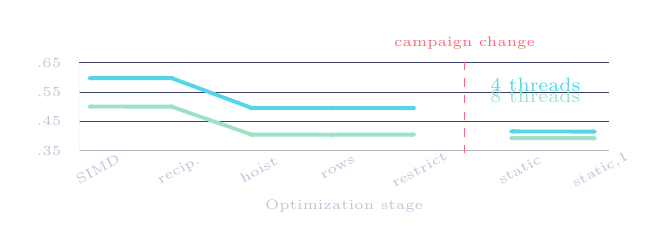
\begin{tikzpicture}[x=1.02cm,y=.62cm]
          \foreach \y/\lab in {0/.35,.6/.45,1.2/.55,1.8/.65} {
            \draw[grid] (-.15,\y) -- (6.45,\y);
            \node[font=\tiny,text=muted,anchor=east] at (-.25,\y) {\lab};
          }
          \draw[white,opacity=.65] (-.15,0) -- (-.15,1.8);
          \draw[white,opacity=.65] (-.15,0) -- (6.45,0);
          \draw[coral,dashed] (4.65,-.05) -- (4.65,1.88);
          \node[font=\tiny,text=coral,anchor=south] at (4.65,1.88) {campaign change};
          \draw[cyan,line width=1.4pt]
            plot coordinates {(0,1.488) (1,1.489) (2,.876) (3,.877) (4,.874)};
          \draw[cyan,line width=1.4pt] plot coordinates {(5.25,.396) (6.25,.392)};
          \draw[mint,line width=1.4pt]
            plot coordinates {(0,.906) (1,.904) (2,.330) (3,.329) (4,.331)};
          \draw[mint,line width=1.4pt] plot coordinates {(5.25,.259) (6.25,.258)};
          \foreach \x/\y in {0/1.488,1/1.489,2/.876,3/.877,4/.874,5.25/.396,6.25/.392}
            \fill[cyan] (\x,\y) circle (.045);
          \foreach \x/\y in {0/.906,1/.904,2/.330,3/.329,4/.331,5.25/.259,6.25/.258}
            \fill[mint] (\x,\y) circle (.045);
          \foreach \x/\lab in {0/SIMD,1/recip.,2/hoist,3/rows,4/restrict,5.25/static,6.25/{static,1}}
            \node[font=\tiny,text=muted,anchor=north,rotate=28] at (\x,-.12) {\lab};
          \node[font=\tiny,text=muted,anchor=north] at (3.15,-.82) {Optimization stage};
          \node[font=\scriptsize,text=cyan,anchor=west] at (4.85,1.35) {4 threads};
          \node[font=\scriptsize,text=mint,anchor=west] at (4.85,1.12) {8 threads};
        \end{tikzpicture}
      \end{beamercolorbox}
    \end{column}
    \begin{column}{.35\textwidth}
      \begin{beamercolorbox}[rounded=true,sep=.18cm,wd=\textwidth]{block body}
        \cardtitle{coral}{IPC AND INSTRUCTION COUNT}
        \footnotesize SIMD $\to$ hoisting cuts retired instructions by
        \textbf{17.6\%} (4 threads) and \textbf{19.8\%} (8 threads), while
        cycles stay close. IPC falls from \textbf{0.598} to \textbf{0.496}
        and from \textbf{0.501} to \textbf{0.405}.
        \smallmuted{Lower IPC here reflects fewer instructions retired, not
        a slowdown by itself.}
        \vspace{.08cm}
        \cardtitle{mint}{STATIC VS. STATIC,1}
        \footnotesize static $\to$ static,1 IPC: \textbf{0.416 $\to$ 0.415} (4 threads),
        \textbf{0.393 $\to$ 0.393} (8 threads); wall-time medians differ by
        less than 0.2\%. No clear winner. \smallmuted{The dashed gap marks
        separate campaigns.}
      \end{beamercolorbox}
    \end{column}
  \end{columns}
\end{frame}

\begin{frame}{Measured comparison: SIMD-only vs. static schedules}
  \eyebrow{RESULTS \quad / \quad 05 \quad N=4000}
  {\smallmuted{Five native \texttt{perf} runs per configuration; bars show median wall time.}}
  \vspace{.12cm}

  \begin{columns}[T,onlytextwidth]
    \begin{column}{.64\textwidth}
      \begin{beamercolorbox}[rounded=true,sep=.18cm,wd=\textwidth]{block body}
        \centering
        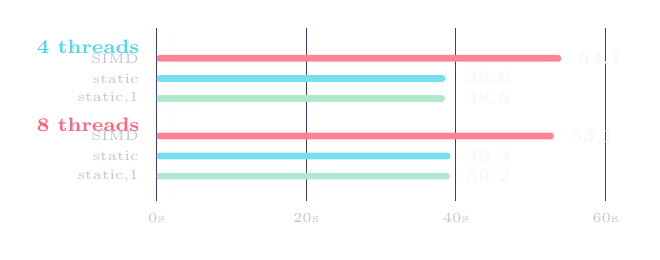
\begin{tikzpicture}[x=.095cm,y=.34cm]
          \foreach \x/\lab in {0/0,20/20,40/40,60/60} {
            \draw[grid] (\x,0) -- (\x,6.45);
            \node[font=\tiny,text=muted,anchor=north] at (\x,-.12) {\lab s};
          }
          \node[font=\scriptsize\bfseries,text=cyan,anchor=east] at (-1,5.75) {4 threads};
          \node[font=\scriptsize\bfseries,text=coral,anchor=east] at (-1,2.85) {8 threads};
          \node[font=\tiny,text=muted,anchor=east] at (-1.1,5.32) {SIMD};
          \draw[fill=coral!80,draw=none,rounded corners=1pt] (0,5.2) rectangle (54.055,5.45);
          \node[font=\scriptsize\bfseries,text=white,anchor=west] at (55,5.32) {54.1};
          \node[font=\tiny,text=muted,anchor=east] at (-1.1,4.57) {static};
          \draw[fill=cyan!80,draw=none,rounded corners=1pt] (0,4.45) rectangle (38.566,4.7);
          \node[font=\scriptsize\bfseries,text=white,anchor=west] at (40,4.57) {38.6};
          \node[font=\tiny,text=muted,anchor=east] at (-1.1,3.82) {static,1};
          \draw[fill=mint!80,draw=none,rounded corners=1pt] (0,3.7) rectangle (38.536,3.95);
          \node[font=\scriptsize\bfseries,text=white,anchor=west] at (40,3.82) {38.5};
          \node[font=\tiny,text=muted,anchor=east] at (-1.1,2.42) {SIMD};
          \draw[fill=coral!80,draw=none,rounded corners=1pt] (0,2.3) rectangle (53.058,2.55);
          \node[font=\scriptsize\bfseries,text=white,anchor=west] at (54,2.42) {53.1};
          \node[font=\tiny,text=muted,anchor=east] at (-1.1,1.67) {static};
          \draw[fill=cyan!80,draw=none,rounded corners=1pt] (0,1.55) rectangle (39.250,1.8);
          \node[font=\scriptsize\bfseries,text=white,anchor=west] at (40,1.67) {39.3};
          \node[font=\tiny,text=muted,anchor=east] at (-1.1,.92) {static,1};
          \draw[fill=mint!80,draw=none,rounded corners=1pt] (0,.8) rectangle (39.188,1.05);
          \node[font=\scriptsize\bfseries,text=white,anchor=west] at (40,.92) {39.2};
          \draw[white,opacity=.65,dashed] (0,3.35) -- (6.2,3.35);
        \end{tikzpicture}
      \end{beamercolorbox}
      \vspace{.12cm}
      \begin{beamercolorbox}[rounded=true,sep=.14cm,wd=\textwidth]{block body}
        \scriptsize
        \textcolor{coral}{SIMD} \quad
        \textcolor{cyan}{static: blocks} \quad
        \textcolor{mint}{static,1: cyclic rows}
        \hfill Seconds; lower is better.
      \end{beamercolorbox}
    \end{column}
    \begin{column}{.34\textwidth}
      \begin{beamercolorbox}[rounded=true,sep=.2cm,wd=\textwidth]{block body}
        \cardtitle{mint}{SPEED-UP VS. SIMD-ONLY}
        \metric{mint}{1.40$\times$}\quad\small 4 threads\\[.04cm]
        \metric{mint}{1.35$\times$}\quad\small 8 threads\\[.08cm]
        \footnotesize Both static schedules vs. SIMD-only.\\[.1cm]
        \cardtitle{coral}{STATIC VS. STATIC,1}
        \footnotesize Static,1 is only \textbf{0.08\%} faster at 4 threads and
        \textbf{0.16\%} at 8 threads; ranges overlap.
        \smallmuted{SIMD and static results come from separate campaigns.}
      \end{beamercolorbox}
    \end{column}
  \end{columns}
\end{frame}

\begin{frame}{How static schedules vary across datasets}
  \eyebrow{DATASET COMPARISON \quad / \quad 06}
  {\smallmuted{Median wall-time change: $(\text{static,1}/\text{static}-1)\times100\%$; negative means static,1 is faster.}}
  \vspace{.14cm}

  \begin{columns}[T,onlytextwidth]
    \begin{column}{.63\textwidth}
      \begin{beamercolorbox}[rounded=true,sep=.2cm,wd=\textwidth]{block body}
        \centering
        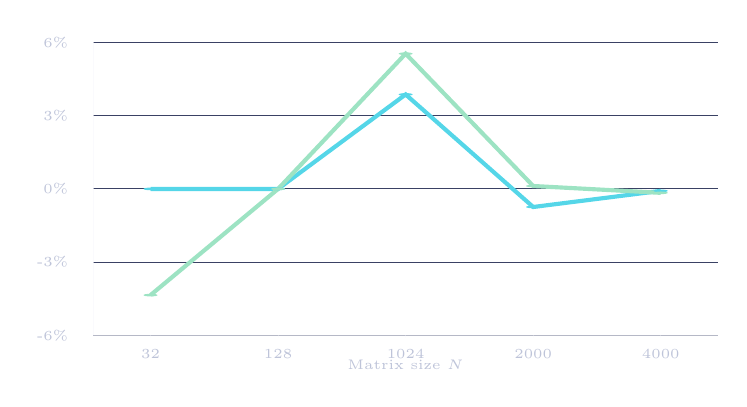
\begin{tikzpicture}[x=1.62cm,y=.31cm]
          \foreach \y/\lab in {-6/-6,-3/-3,0/0,3/3,6/6} {
            \draw[grid] (.55,\y) -- (5.45,\y);
            \node[font=\tiny,text=muted,anchor=east] at (.43,\y) {\lab\%};
          }
          \draw[white,opacity=.65] (.55,-6) -- (.55,6);
          \draw[white,opacity=.65] (.55,-6) -- (5.45,-6);
          \foreach \x/\lab in {1/32,2/128,3/1024,4/2000,5/4000} {
            \draw[white,opacity=.3] (\x,-6) -- (\x,-6.12);
            \node[font=\tiny,text=muted,anchor=north] at (\x,-6.2) {\lab};
          }
          \draw[cyan,line width=1.5pt]
            plot coordinates {(1,0) (2,0) (3,3.87) (4,-.74) (5,-.08)};
          \draw[mint,line width=1.5pt]
            plot coordinates {(1,-4.35) (2,0) (3,5.54) (4,.12) (5,-.16)};
          \foreach \x/\y in {1/0,2/0,3/3.87,4/-.74,5/-.08}
            \fill[cyan] (\x,\y) circle (.055);
          \foreach \x/\y in {1/-4.35,2/0,3/5.54,4/.12,5/-.16}
            \fill[mint] (\x,\y) circle (.055);
          \node[font=\tiny,text=muted,anchor=north] at (3,-6.62) {Matrix size $N$};
        \end{tikzpicture}
        \vspace{.05cm}
        \scriptsize\textcolor{cyan}{4 threads}\qquad
        \textcolor{mint}{8 threads}\qquad
        \textcolor{muted}{positive: static,1 slower}
      \end{beamercolorbox}
    \end{column}
    \begin{column}{.34\textwidth}
      \begin{beamercolorbox}[rounded=true,sep=.2cm,wd=\textwidth]{block body}
        \cardtitle{coral}{WHAT CHANGES WITH $N$?}
        \small At $N=1024$, static,1 is 3.9\% slower (4 threads) and 5.5\% slower
        (8 threads) by the medians.
        \vspace{.12cm}

        \small At $N=4000$, the medians differ by less than 0.2\%.
        \vspace{.12cm}

        \smallmuted{The min--max ranges overlap for every dataset/thread
        pair. The small-$N$ timings are especially sensitive to process
        overhead and timer resolution.}
      \end{beamercolorbox}
    \end{column}
  \end{columns}
  \vspace{.12cm}
  \centering\color{muted}\tiny Five \texttt{perf} runs per setting; medians
  shown; no formal significance test was performed.
\end{frame}

\begin{frame}{Takeaways — and the hand-off to blocked LU}
  \eyebrow{CONCLUSIONS \quad / \quad 07}
  \vspace{.05cm}
  \begin{columns}[T,onlytextwidth]
    \begin{column}{.32\textwidth}
      \begin{beamercolorbox}[rounded=true,sep=.2cm,wd=\textwidth,ht=2.15cm]{block body}
        \cardtitle{cyan}{WHAT CHANGED}
        \small Reciprocal reuse, loop-invariant hoisting, row pointers,
        \texttt{restrict}, and explicit static scheduling build on SIMD.
      \end{beamercolorbox}
    \end{column}
    \begin{column}{.32\textwidth}
      \begin{beamercolorbox}[rounded=true,sep=.2cm,wd=\textwidth,ht=2.15cm]{block body}
        \cardtitle{mint}{WHAT WE OBSERVED}
        \small Static/static,1 medians are close. Static,1 does not show a meaningful,
        consistent improvement over static blocks in these runs.
      \end{beamercolorbox}
    \end{column}
    \begin{column}{.32\textwidth}
      \begin{beamercolorbox}[rounded=true,sep=.2cm,wd=\textwidth,ht=2.15cm]{block body}
        \cardtitle{coral}{WHAT WE CANNOT CLAIM}
        \small Campaigns differ; the input is singular and the timing includes
        the whole process. Results are exploratory, not a correctness claim.
      \end{beamercolorbox}
    \end{column}
  \end{columns}

  \vspace{.25cm}
  \begin{beamercolorbox}[rounded=true,sep=.22cm,wd=\textwidth]{block body}
    \cardtitle{lavender}{NEXT: CHANGE THE ALGORITHM'S GRANULARITY}
    \begin{columns}[T,onlytextwidth]
      \begin{column}{.72\textwidth}
        \small The next section moves from element/row-level tuning to a
        \textbf{tiled LU}: blocks improve data reuse and expose task-level
        parallelism. Dependencies between panel factorization, triangular
        solves, and Schur-complement updates must still be respected.
      \end{column}
      \begin{column}{.26\textwidth}
        \centering
        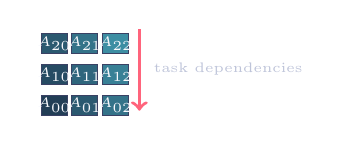
\begin{tikzpicture}[x=.39cm,y=.39cm]
          \foreach \x in {0,1,2} {
            \foreach \y in {0,1,2} {
              \pgfmathsetmacro{\shade}{int(20+14*\x+7*\y)}
              \draw[fill=cyan!\shade!panel,draw=grid] (\x,\y) rectangle ++(.85,.65);
              \node[font=\tiny,text=white] at (\x+.425,\y+.325) {$A_{\y\x}$};
            }
          }
          \draw[->,coral,line width=1.2pt] (3.2,2.8) -- (3.2,.15);
          \node[font=\tiny,text=muted,anchor=west] at (3.35,1.5) {task dependencies};
        \end{tikzpicture}
      \end{column}
    \end{columns}
  \end{beamercolorbox}

  \vspace{.19cm}
  \centering{\color{cyan}\large\bfseries From optimizing the update loop \quad
  $\longrightarrow$ \quad improving reuse across blocks}
\end{frame}

\end{document}
